\documentclass{beamer}
\usepackage[T1]{fontenc}
\usepackage{textcomp}
\usepackage{ucs}
\usepackage[utf8x]{inputenc}
\usepackage[ngerman]{babel}
\usepackage{lmodern}
\usepackage{graphicx}
\usepackage{amsmath, amssymb, amsthm, array, ulem}
\usepackage{beamerthemesplit}
\usepackage{hyperref} % Zur Darstellung von URLs

\beamersetuncovermixins{\opaqueness<1>{25}}{\opaqueness<2->{15}}

\begin{document}
\title[Antz: Ameisenkolonie-Optimierung]{Antz: Ameisenkolonie-Optimierung} 
\subtitle{Software-Projekt 2}
\author{Bernhard Fuchs, Florian Müller} 
\date{4. Juni 2014} 

\frame{\titlepage} 

\frame[shrink]{
  \frametitle{Agenda}
  \vspace{10px}
  \tableofcontents
} 



\section{Einführung}
\frame{
  \frametitle{Überblick}
  \begin{itemize}
    \item Thema: Ameisenalgorithmus zum Finden kürzester Pfade
    \item Technologie: Python mit pyGame (Simulation mit graphischem  Interface)
    \item Fokus der Applikation
    \item Ameisenkolonie-Optimierung
    \begin{itemize}
	  \item Verhalten natürlicher Ameisen auf Futtersuche
	  \item Konzentration des Duftstoffs Pheromon $\rightarrow$ Ameisenstrasse
	  \item Übertragung auf Algorithmus (modellbasierte Suche)
    \end{itemize}
  \end{itemize}
}



\frame{
\frametitle{Hilfsmittel/Vorgehen}
  \begin{itemize}
    \item Tools erwähnen
    \item ??? (folgt)
  \end{itemize}
}

\section{Algorithmus}

\subsection{Grober Ablauf}

\frame{
	\frametitle{Grober Ablauf}
	\begin{enumerate}
	\item Exploration - Entdecken
		\begin{itemize}
		\item Ameise sucht Futter
		\item Nimmt Kanten mit mehr Pheromonen
		\end{itemize}
	\pause
	\item Exploitation - Verwertung
		\begin{itemize}
		\item Ameise geht zurück zum Nest
		\item Erhöht Pheromonmenge auf Kanten
		\end{itemize}	
	\pause
	\item Evaporation - Verdunstung
		\begin{itemize}
		\item Der Pheromongehalt auf allen Kanten wird reduziert
		\end{itemize}	
	\end{enumerate}
}
\section{Step By Step}

\frame{
	\frametitle{Step By Step Durchlauf}
	\begin{figure}
		\includegraphics<1>[width=0.8\textwidth]{img/antz-step-1.png}
		\includegraphics<2>[width=0.8\textwidth]{img/antz-step-2.png}
		\includegraphics<3>[width=0.8\textwidth]{img/antz-step-3.png}
		\includegraphics<4>[width=0.8\textwidth]{img/antz-step-4.png}
		\includegraphics<5>[width=0.8\textwidth]{img/antz-step-5.png}
		\includegraphics<6>[width=0.8\textwidth]{img/antz-step-6.png}
		\includegraphics<7>[width=0.8\textwidth]{img/antz-step-7.png}
		\includegraphics<8>[width=0.8\textwidth]{img/antz-step-8.png}
		\includegraphics<9>[width=0.8\textwidth]{img/antz-step-9.png}
	\end{figure}
}

\subsection{Berechnungen}

\frame{
	\frametitle{Berechnungen}
	\begin{description}
		\item [Kantenauswahl] $p_{k_i} = \frac{phero_{k_i}^\alpha \cdot
		cost_{k_i}^\beta}{\sum\nolimits_{i=0}^n phero_{k_i}^\alpha \cdot
		cost_{k_i}^\beta}$ \pause
		\item [Pheromon-Update] $phero = phero +
		\left({\frac{1}{pathlength}}\right)^\gamma$  \pause
		\item [Pheromon-Evaporation] $phero = phero \cdot \left({ 1 -
\frac{phero_{k_i}}{phero_{max}}}\right)^\delta$
	\end{description}
}

\frame{
	\frametitle{Gewichtete Wahrscheinlichkeit}
	
	Beispiel: Kanten $\{K_1, K_2\}$; $phero_{k_1} = 5; phero_{k_2} = 10; \alpha =
2; \beta = 0$ 
	
	\[ p_{k_i} = \frac{phero_{k_i}^\alpha \cdot
			cost_{k_i}^\beta}{\sum\nolimits_{i=0}^n phero_{k_i}^\alpha \cdot
			cost_{k_i}^\beta} \]
	
	\only<1>{Alle Wahrscheinlichkeiten berechnen:}
	\only<2>{Gewichtung:}
	
	\begin{itemize}
		\only<1>{
			\item $p_{k_1} = \frac{5^2 (\cdot 1)}{5^2 + 10^2} = 0.2$
			\item $p_{k_2} = \frac{10^2 (\cdot 1)}{5^2 + 10^2} = 0.8$
		}
		\only<2>{
			\item $gew = (p_{k_1}, p_{k_1} + p_{k_2}) = (0.2, 1)$
			\item $r = random.random() = 0.46$
			\item $tuple_{index} = bisect(gew, r) = 1$
			\item $r$ öfters zwischen $0.2$ und $1$, manchmal zwischen $0$ und $0.2$
		}
	\end{itemize}
}

\frame{
	\frametitle{Einflussnahme}
	
	\only<1-2>{
		\begin{description}
		\item [$\alpha$] Verstärkung der Unterschiede zwischen Pheromonwerten \pause
		\item [$\beta$] Verstärkung der Unterschiede zwischen Kosten und Gewichtung
von Kosten
		\end{description}
	}
	
	\only<3-6>{
		\only<3-5>{
			\[ p_{k_i} = \frac{phero_{k_i}^\alpha \cdot
					cost_{k_i}^\beta}{\sum\nolimits_{i=0}^n phero_{k_i}^\alpha \cdot
					cost_{k_i}^\beta} \]
		}
	
		\only<3>{
			\begin{itemize}
			\item Alle Werte werden zwischen 0 und 1 normiert
			\item $phero_1 = 0.7; phero_2 = 0.3; cost_1 = 0.8; cost_2 = 0.5$
			\end{itemize}
		}
		
		\only<4>{
			\begin{itemize}
			\item Mit $\alpha = 1; \beta = 1$
			\end{itemize}
			
			\[ p_1 = \frac{0.7^1 \cdot 0.8^1}
				{0.7^1 \cdot 0.8^1 + 0.3^1 \cdot 0.5^1} = 0.79 \]
			\[ p_2 = \frac{0.3^1 \cdot 0.5^1}
				{0.7^1 \cdot 0.8^1 + 0.3^1 \cdot 0.5^1} = 0.21 \]
		}

		\only<5>{
			\begin{itemize}
			\item Mit $\alpha = 2; \beta = 2$
			\end{itemize}
			
			\[ p_1 = \frac{0.7^2 \cdot 0.8^2}
				{0.7^2 \cdot 0.8^2 + 0.3^2 \cdot 0.5^2} = 0.93 \]
			\[ p_2 = \frac{0.3^2 \cdot 0.5^2}
				{0.7^2 \cdot 0.8^2 + 0.3^2 \cdot 0.5^2} = 0.07 \]
		}
		
		\only<6>{
			\framesubtitle{Fazit}
			\begin{itemize}
			\item Die Unterschiede haben sich verstärkt.
			\item Die Wahrscheinlichkeit ist grösser, dass die Ameise $p_1$ wählt.
			\end{itemize}
		}
	}
}

\subsection{Dijstra und Konfigurationswerte}

\frame{
	\frametitle{Dijstra und Konfigurationswerte}
	
	\begin{itemize}
	\item Bei 500 Hops von Nest zu Food
	\end{itemize}
	
	\begin{minipage}[t]{\textwidth}
		\tiny
		\csvautotabular[separator=semicolon]{dijkstra-ants.csv}
	\end{minipage}
}

\section{Applikation}

\frame{
	\frametitle{Aufbau}
	\begin{figure}
		\begin{minipage}[t]{0.4\textwidth}
			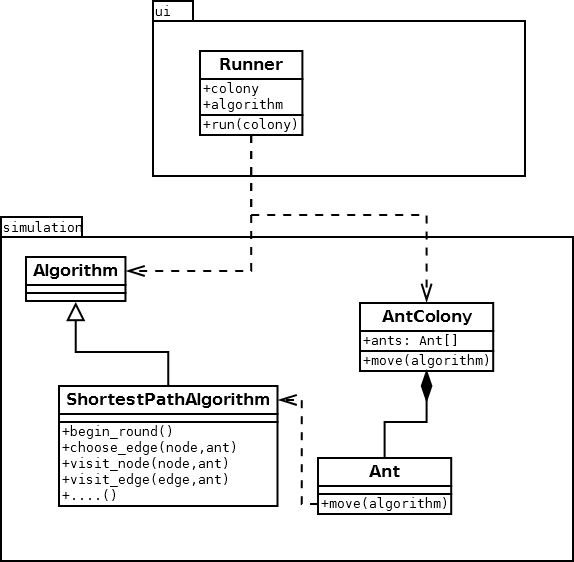
\includegraphics[width=\textwidth]{img/uml-short.png}
		\end{minipage}
		\begin{minipage}[t]{0.4\textwidth}
			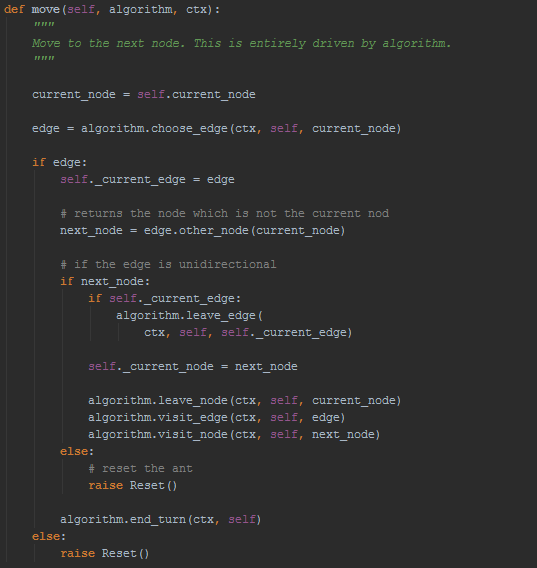
\includegraphics[width=\textwidth]{img/ant-code.png}
		\end{minipage}
	\end{figure}
}

\section{Fazit und Ausblick}
\frame{ 
\frametitle{Fazit und Ausblick}
\begin{large}\textbf{Erkenntnisse}\end{large}
\begin{itemize}
\item ACO-Algorithmus beim Finden des kürzesten Pfades oft recht langsam und mit suboptimaler Lösungsfindung (im Vergleich zu Dijkstra oder A*)
\item Rasche Anpassung an veränderte Gegebenheiten (Hindernisse)
\item Zeitintensiv: Anpassung an Parameter; Refactorings
\item Fokus gezielter vornehmen
\end{itemize}
\begin{large}\textbf{Ausblick}\end{large}
\begin{itemize}
\item Stärkere Angleichung an die Realität (z.B. mehrere Kolonien; Feinde; Überlebensstrategien)
\item Optimierung der Performance
\item Integration von Lösungen für weitere Probleme (z.B. TSP)
\end{itemize}}



\frame{
\frametitle{Wichtige Literatur}
\begin{footnotesize}
\begin{itemize}
	\item Merkle, D.: \textit{Ameisenalgorithmen: Optimierung und Modellierung}, Diss. Karlsruhe 2002.
	\item Dorigo, M.; Stützle, Th.: \textit{Ant Colony Optimization}, Cambridge, MA 2004.
	\item Schiller, D.: \textit{Kombinatorische Optimierung mit Ameisensystemen}, Seminararbeit, Köln 2008.	
	\item Santoso, L. W.; Setiawan, A.;Prajogo, A. K.: \textit{Performance Analysis of Dijkstra, A* and Ant Algorithm for Finding Optimal Path Case Study: Surabaya City Map}, Surabaya 2011.
\end{itemize}
\end{footnotesize}
}



\frame{
\frametitle{Fragen und Diskussion}
\begin{Large}Fragen? – Let's talk!\end{Large}
}


\end{document}
